\documentclass[handout, aspectratio=169, 10pt]{beamer}

% packages
\usepackage{newpxmath} % math font is Palatino compatible
% \usepackage[nomath]{fontspec}

\usepackage{setspace}
\usepackage{xcolor}
\usepackage{soul} % for \st
\usepackage{hyperref} % for links
\definecolor{links}{HTML}{2A1B81}
\hypersetup{colorlinks,linkcolor=,urlcolor=links}


% table stuff
\usepackage{chronosys}
\usepackage{verbatim}
% \pagenumbering{arabic}
\usepackage{tabularx}
\usepackage{booktabs}
\usepackage{ragged2e}
\usepackage{mathtools}

% R Code
\usepackage{listings}
\usepackage{courier}
\lstset{basicstyle=\scriptsize\ttfamily,breaklines=true}
\lstset{framextopmargin=50pt,frame=bottomline}

% themes
\usetheme[progressbar=frametitle, block=fill]{metropolis}
\useoutertheme{metropolis}
\useinnertheme{metropolis}

% colors
\definecolor{dimwhite}{rgb}{0.99, 0.99, 0.99}
\definecolor{charcoal}{rgb}{0.21, 0.27, 0.31}
\definecolor{slategray}{rgb}{0.44, 0.5, 0.56}
\definecolor{dimgray}{rgb}{0.41, 0.41, 0.41}
\definecolor{bleudefrance}{rgb}{0.19, 0.55, 0.91}

% beamer options
\setbeamercolor{author}{fg=charcoal}
\setbeamercolor{background canvas}{bg=white}
\setbeamercolor{section in toc}{fg=charcoal}
\setbeamercolor{subsection in toc}{fg=dimgray}
\setbeamercolor{frametitle}{bg=dimwhite, fg=charcoal}
\setbeamercolor{progress bar}{fg=slategray, bg=fg!50!black!30}
\setbeamercovered{transparent}
\setbeamertemplate{itemize items}[triangle]
\setbeamertemplate{itemize subitem}[circle]
\setbeamertemplate{itemize subsubitem}[square]
\setbeamersize{text margin left=7mm,text margin right=7mm} 

% new commands
\newcommand{\q}[1]{``#1''}
\newcommand{\hs}[1]{\textsc{\hfill\scriptsize\color{dimgray}#1}}
\newcommand{\g}[1]{{\color{gray}#1}}
\newcommand{\dg}[1]{{\color{dimgray}#1}}
\newcommand{\sg}[1]{{\color{slategray}#1}}
\newcommand{\bdf}[1]{{\color{bleudefrance}#1}}
\newcommand{\itemcolor}[1]{\renewcommand{\makelabel}[1]{\color{#1}\hfil ##1}}
\newcommand\Wider[2][2em]{
\makebox[\linewidth][c]{
  \begin{minipage}{\dimexpr\textwidth+#1\relax}
  \raggedright#2
  \end{minipage}
  }
}

% misc
\linespread{1.35}

% Math stuff
\newcommand{\norm}[1]{\left\lVert#1\right\rVert}
\newcommand{\R}{\mathbb{R}}
\newcommand{\E}{\mathbb{E}}
\newcommand{\V}{\mathbb{V}}
\newcommand{\probP}{\text{I\kern-0.15em P}}
\newcommand{\ol}{\overline}
%\newcommand{\ul}{\underline}
\newcommand{\pp}{{\prime \prime}}
\newcommand{\ppp}{{\prime \prime \prime}}
\newcommand{\policy}{\gamma}
\newcommand{\plim}{ \overset{p}{\to}}
\newcommand{\hnot}{ \overset{H_0}{\to}}

% Causal Graphs
\usetikzlibrary{shapes,decorations,arrows,calc,arrows.meta,fit,positioning}
\tikzset{
    -Latex,auto,node distance =1 cm and 1 cm,semithick,
    state/.style ={ellipse, draw, minimum width = 0.7 cm},
    point/.style = {circle, draw, inner sep=0.04cm,fill,node contents={}},
    bidirected/.style={Latex-Latex,dashed},
    el/.style = {inner sep=2pt, align=left, sloped}
}
\title{Discrete Chocice Models: Individual Data}
\author{Chris Conlon}
\institute{NYU Stern: Applied Econometrics}

\date{Spring 2023}

\begin{document}

\frame{\titlepage}


\begin{frame}{Readings}
After class please read:
\begin{itemize}
\item Ken Train \url{https://eml.berkeley.edu/books/choice2.html}
\begin{itemize}
\item Chapters 1-6
\end{itemize}
\end{itemize}
\end{frame}




\begin{frame}{Lots of Discrete Choices (in IO and elsewhere)}
\begin{itemize}
\item Choosing a brand from the supermarket
\item Choosing a hospital
\item Choosing a school/major
\item Choosing where to live
\end{itemize}
\end{frame}



\begin{frame}{A Purely Statistical Setup: Utility}
An individual $i$ has utility for choice $j$:
\begin{align*}
u_{ij} = V_{ij}(\theta) + \varepsilon_{ij}
\end{align*}
Idea:
\begin{itemize}
\item Make some assumption on $f(\varepsilon_{ij})$
\item Estimate $V_{ij}(\theta)$
\end{itemize}
\end{frame}

\begin{frame}{A Purely Statistical Setup: Choice Probabilities}
Consider the \alert{choice probability}
\begin{align*}
s_{ij}(\theta)=\mathbb{P}(u_{ij} > u_{ik};\, \forall k \neq j)
\end{align*}
Idea:
\begin{itemize}
\item Only choose $j$ if it is preferred to all options $k$.
\item Helpful to assume that $f(\varepsilon_{ij})$ is continuous and full support so that ties are measure zero.
\end{itemize}
\end{frame}


\begin{frame}{A Purely Statistical Setup: Data}
Assume that we see individual $i$ makes a:
\begin{itemize}
\item Mutually exclusive and exhaustive discrete choice.
\item $y_{ij} \in \{0,1\}$ and $\sum_{k} y_{ik} =1$
\end{itemize}
 And that we observe $y_{ij}$ for $i=1,\ldots,N$ and all $j$. We can write the likelihood of the dataset as 
\begin{align*}
L(\theta) &= \prod_{i} \prod_j s_{ij}^{y_{ij}}(\theta)\\
\ell(\theta) &= \sum_{i} \sum_j y_{ij} \log   s_{ij}(\theta)
\end{align*}
Since the cases where $y_{ij}=0$ do not contribute to $\ell(\theta)$ some people abuse notation and drop $y_{ij}$ or $\sum_j$ and write $\ell(\theta) = \sum_{i: y_{ij}=1} \log s_{ij}(\theta)$ (but let's not do that).
\end{frame}


\begin{frame}
\frametitle{A Purely Statistical Setup: Parametric Forms}
In order to compute the choice probabilities, we must perform a $J$ dimensional integral over $f(\boldsymbol{\varepsilon_i})$.
\begin{align*}
s_{ij} =  \int \mathbb{I}( \varepsilon_{ij}-\varepsilon_{ik} > V_{ik} - V_{ij} ) f( \boldsymbol{\varepsilon_i}) \partial \boldsymbol{\varepsilon_i }
\end{align*}
There are some choices that make our life easier
\begin{itemize}
\item Multivariate normal: $\varepsilon_i  \sim \mathcal{N}(0,\Omega)$. $\longrightarrow$ \alert{ multinomial probit}.
 \item Gumbel/Type 1 EV: $f(\varepsilon_{ij}) = e^{-\varepsilon_{ij}}  e^{-e^{-\varepsilon_{ij}}}  $ and $F(\varepsilon_{ij}) = 1- e^{-e^{-\varepsilon_{ij}}}$ $\longrightarrow$ \alert{multinomial logit}
 \item There are also heteroskedastic variants of the Type I EV/ Logit framework.
\end{itemize}
\end{frame}

\begin{frame}{Parametric Forms: Multinomial Probit}
Multinomial Probit?
\begin{itemize}
\item The probit has $\boldsymbol{\varepsilon_i} \sim \mathcal{N}(0,\Sigma)$.
\item If $\Sigma$ is unrestricted, then this can produce relatively flexible substitution patterns.
\item Flexible is relative: still have normal tails, only pairwise correlations, etc.
\item It might be that $\rho_{12}$ is large if $1,2$ are similar products.
\item Much more flexible than Logit
\end{itemize}
Downside
\begin{itemize}
\item $\Sigma$ has potentially $J^2$ parameters (that is a lot)!
\item Maybe $J * (J-1)/2$ under symmetry. (still a lot).
\item Each time we want to compute $s_{ij}(\theta)$ we have to simulate an integral of dimension $J$.
\item I wouldn't do this for $J \geq 5$.
\end{itemize}
\end{frame}


\begin{frame}{Multinomial Logit}
Multinomial Logit has closed form choice probabilities
\begin{align*}
s_{ij} = \frac{e^{V_{ij}}}{\sum_k e^{V_{ik}}} %\approx \frac{e^{\beta' x_{ij}}}{\sum_k e^{\beta' x_{ik}}}
\end{align*}
 Expected maximum also has closed form:
\begin{align*}
\E[\max_j u_{ij}] = \log \left(\sum_j \exp[V_{ij}] \right) + \gamma
\end{align*}
Logit Inclusive Value is helpful for several reasons
\begin{itemize}
\item Expected utility of best option (without knowledge of $\varepsilon_i$) does not depend on $\varepsilon_{ij}$.
\item This is a globally concave function in $V_{ij}$ (more on that later).
\item Allows simple computation of $\Delta CS$ for consumer welfare (but not $CS$ itself).
\end{itemize}
\end{frame}

\section{Properties of Logit}


\begin{frame}
\frametitle{Multinomial Logit: Identification}
What is actually identified here?
\begin{itemize}
\item Helpful to look at the ratio of two choice probabilities
\begin{align*}
\log \frac{s_{ij}(\theta)}{s_{ik}(\theta)} 
&= V_{ij} - V_{ik}
\end{align*}
\item We only identify the \alert{difference in indirect utilities} not the levels.
\item This is a feature and not a bug. Why?
\end{itemize}
\end{frame}

\begin{frame}
\frametitle{Multinomial Logit: Identification}
As another idea suppose we add $C$ to each $V_{ij}$:
\begin{align*}
s_{ij} = \frac{e^{C+ V_{ij}} }{\sum_k e^{C + V_{ik}}} 
       = \frac{e^C e^{ V_{ij}} }{\sum_k e^C e^{V_{ik}}}
       =\frac{\exp^{V_{ij}} }{\sum_k \exp^{ V_{ik}}} 
\end{align*}
This has no effect.  That means we need to fix a normalization $C$.\\
\begin{itemize}
\item We normalize one of the choices to provide a utility of zero $V_{ik}-\underbrace{V_{ik}}_{=C}=0$
\item We actually already made another normalization. Does anyone know which?
\end{itemize}
\end{frame}


\begin{frame}
\frametitle{Multinomial Logit: Identification}
The most sensible normalization in many settings is to allow for an \alert{outside option} which produces no utility in expectation.
\begin{align*}
s_{ij} = \frac{e^{V_{ij}}}{1+\sum_k e^{V_{ik} }} 
\end{align*}
\begin{itemize}
\item Hopefully the choice of outside option is well defined: not buying a yogurt, buying some other used car, etc.
\item Now this resembles the binomial logit model more closely.
\end{itemize}
\end{frame}


\begin{frame}{Back to Scale of Utility}
\begin{itemize}
\item Consider $U_{ij}^{*} = V_{ij} + \varepsilon_{ij}^{*}$ with $Var(\varepsilon^{*}) = \sigma^2 \pi^2/6$.
\item Without changing behavior we can divide by $\sigma$ so that $U_{ij} = V_{ij}/\sigma + \varepsilon_{ij}$ and $Var(\varepsilon^{*}/\sigma)=Var(\varepsilon) = \pi^2/6$
\begin{align*}
s_{ij} = \frac{e^{V_{ij}/\sigma}}{\sum_k e^{V_{ik}/\sigma}} \approx \frac{e^{\beta^{*}/\sigma \cdot x_{ij}}}{\sum_k e^{\beta^{*}/\sigma \cdot x_{ik}}}
\end{align*}
\item Every coefficient $\beta$ is rescaled by $\sigma$. This implies that only the ratio $\beta^{*}/\sigma$ is identified. 
\item Coefficients are relative to variance of unobserved factors. More unobserved variance $\longrightarrow$ smaller $\beta$.
\item Ratio $\beta_1/\beta_2$ is invariant to the scale parameter $\sigma$.
\end{itemize}
\end{frame}


\begin{frame}
\frametitle{Multinomial Logit: Elasticity}
An important output from a demand system are elasticities w.r.t $x_{ij}$
\begin{align*}
\frac{\partial s_{ij}}{\partial x_{ij}} = \beta \cdot \left(\mathbb{I}[j = k]\cdot s_{ij} - s_{ij}\cdot s_{ik} \right)
\end{align*}
\begin{itemize}
\item This implies that $ \eta_{jj}^x = \frac{\partial s_{ij}}{\partial x_{ij}} \frac{x_{ij}}{s_{ij}}  = \beta x_{ij} (1-s_{ij})$.
\item  $ \eta_{jk}^x = \frac{\partial s_{ij}}{\partial x_{ik}} \frac{x_{ik}}{s_{ij}}  = -\beta x_{ik} s_{ik}$.

\item The own elasticity is increasing in own $x_{ij}$!
\begin{itemize}
\item Why is this a bad idea? What if $x_{ij}$ is the price of $j$??
\end{itemize}
\item The cross elasticity doesn't depend on which product $j$ you are talking about!
\end{itemize}
\end{frame}


\begin{frame}
\frametitle{Multinomial Logit: Substitution}
I prefer to characterize substitution via diversion ratios
\begin{align*}
\frac{\partial s_{ij}}{\partial x_{ij}} &=\left(\mathbb{I}[j = k]\cdot s_{ij} - s_{ij}\cdot s_{ik} \right)\\
D_{jk} &= \frac{\partial s_{ik}}{\partial x_{ij}} / \left|\frac{\partial s_{ij}}{\partial x_{ij}}\right| = \frac{s_{ik}}{1-s_{ij}}
\end{align*}
\begin{itemize}
\item Second choices: $\mathbb{P}\left(i \text { chooses } k \in \mathcal{J} \setminus \{j\} \mid i \text { chooses } j \in \mathcal{J} \right) =\frac{s_{ik}}{1-s_{ij}}$
\item Whether we increase/reduce $x_{ij}$ or remove $j$ from choice set, we get the same substitution patterns.
\item Substitution is \alert{proportional to share}.
\end{itemize}
\end{frame}


\begin{frame}
\frametitle{Multinomial Logit: Estimation Details}
Maximum (log)-likelihood:
\begin{align*}
\max_{\theta} \ell(\theta) &= \sum_{i} \sum_j y_{ij} \log   s_{ij}(\theta)
\end{align*}
Hard part is computing the \alert{scores}:
\begin{align*}
\frac{\partial \, \log   s_{ij}(\theta)}{\partial\, \theta} = s_{ij} \cdot (1-s_{ij}) \cdot \frac{\partial V_{ij}}{\partial \theta}
\end{align*}
\end{frame}



\begin{frame}
\frametitle{Multinomial Logit: Estimation Details}
Method of Moments with some \alert{instruments} $z_{ij}$:
\begin{align*}
 \sum_{i} \sum_j \left[y_{ij} -  s_{ij}(\theta) \right] z_{ij}=0
\end{align*}
It turns out the best choice for $z_{ij}$ is the \alert{score} (evaluated at true $\theta_0$):
\begin{align*}
z_{ij} = \frac{\partial \, \log   s_{ij}(\theta)}{\partial\, \theta} = s_{ij} \cdot (1-s_{ij}) \cdot \frac{\partial V_{ij}}{\partial \theta}
\end{align*}
Why? this attains the semi-parametric efficiency bound (see Chamberlain 1987).
\end{frame}


\begin{frame}
\frametitle{Multinomial Logit: Estimation Details}
Method of Moments with some \alert{instruments} $z_{ij}$:
\begin{align*}
 \sum_{i} \sum_j \left[y_{ij} -  s_{ij}(\theta) \right] z_{ij}=0
\end{align*}
It turns out the best choice for $z_{ij}$ is the \alert{score} (evaluated at true $\theta_0$):
\begin{align*}
z_{ij} = \frac{\partial \, \log   s_{ij}(\theta)}{\partial\, \theta} = s_{ij} \cdot (1-s_{ij}) \cdot \frac{\partial V_{ij}}{\partial \theta}
\end{align*}
Why? this attains the semi-parametric efficiency bound (see Chamberlain 1987).
\end{frame}




\begin{frame}
\frametitle{Estimation Details: Softmax}
Statistics/Computer Science offer an alternative interpretation of $\log \sum_j \exp$
\begin{itemize}
\item Sometimes this is called \alert{softmax} function .
\item Think of this as a continuous/concave approximation to the maximum.
\item Consider $\max\{x,y\}$ vs $\log(\exp(x) + \exp(y))$. The $\exp$ exaggerates the differences between $x$ and $y$ so that the larger term dominates.
\item We can accomplish this by rescaling $k$:  $\log(\exp(kx) + \exp(ky))/k$ as $k$ becomes large the derivatives become infinite and this approximates the ``hard'' maximum.
\item $g(1, 2) = 2.31$, but $g(10, 20) = 20.00004$.
\end{itemize}
But be \alert{careful} about how you code this. $e^{300}$ may be too large for your computer!
\end{frame}

\begin{frame}{Estimation Details: Softmax}
\begin{figure}[htbp]
\begin{center}
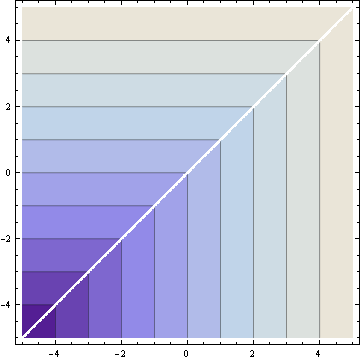
\includegraphics[width=2in]{./resources_1/hardmax.png}
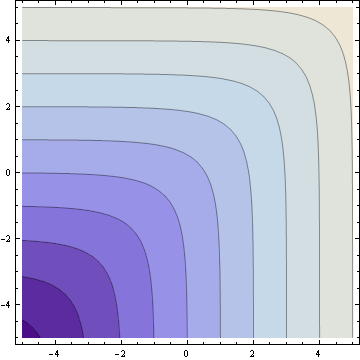
\includegraphics[width=2in]{./resources_1/softmax.png}
\end{center}
\end{figure}
\end{frame}


\section{Thanks!}


\end{document}
